\subsection{Сценарий 3: Simple World Communication} \label{exp-results-svc}

Были построены графики вознаграждений и согласованности коммуникаций для двух преследователей и одной жертвы в сценарии Simple World Communication, которые представлены на \firef{fig:result-swc-rew} и \firef{fig:result-swc-comm}. На этих графиках зелёная кривая~--- это результат обучения MADDPG, а серая~--- DDPG.

\begin{figure}[ht!]
    \center
    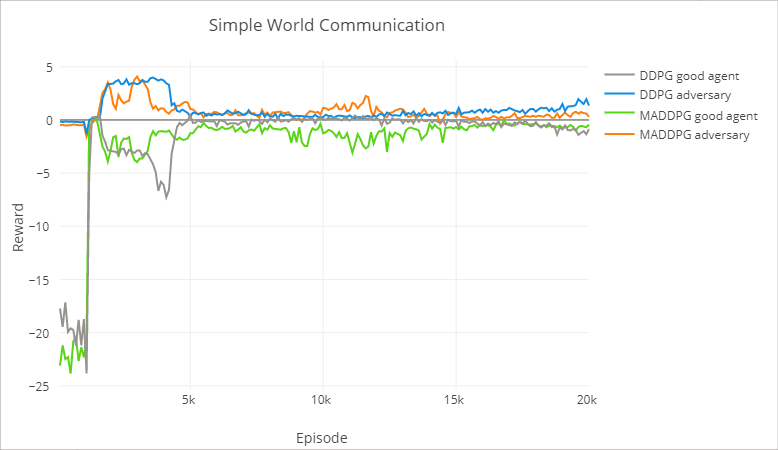
\includegraphics [scale=0.6] {my_folder/images/ch5/swc-rew.png}
    \caption{Среднее вознаграждение преследователей и жертвы с алгоритмами DDPG и MADDPG}
    \label{fig:result-swc-rew}
\end{figure}

\begin{figure}[ht!]
    \center
    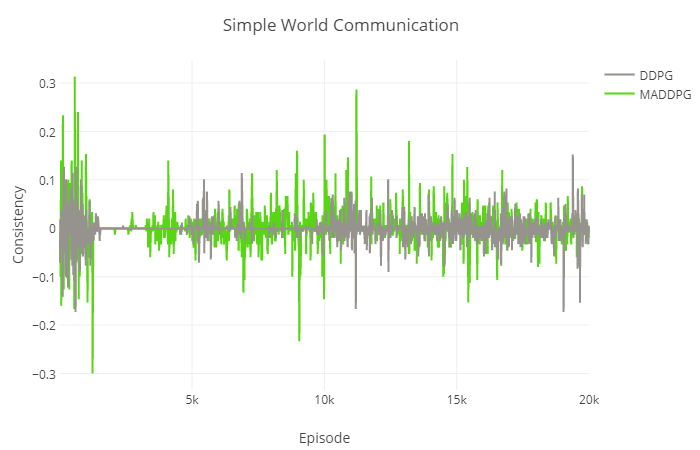
\includegraphics [scale=0.6] {my_folder/images/ch5/swc-comm.png}
    \caption{График консистентности действий коммуникации для алгоритмов DDPG и MADDPG}
    \label{fig:result-swc-comm}
\end{figure}

К сожалению, из-за ограниченности времени и вычислительных ресурсов нам не удалось добиться сходимости консистентности действий общения в этом сценарии, это видно на \firef{fig:result-swc-comm}. Из графика видно, что отклонения от нуля больше в случае MADDPG, но этого оказалось недостаточно для того, чтобы «закрепить результат», научиться преследователю использовать получаемые сигналы лидера так, чтобы улучшить общее вознаграждение.

Вследствие чего результаты алгоритма MADDPG ничем не выделяются по сравнению с DDPG, это можно видеть на \firef{fig:result-swc-rew}.

Также в этом сценарии трудно установить «конец игры», когда цель достигнута, так как во время обучения агенты обеих команд постепенно действуют всё более адекватно, однако это трудно увидеть на графике среднего вознаграждения. То преследователи изобретают более-менее эффективную тактику, и получают большую награду, то жертва обучается на своих ошибках и начинает учитывать это. Однако, на рендеринге можно видеть, что и преследователи, и жертва ведут себя вполне адекватно. Преследователи догоняют жертву, жертва убегает и, по возможности, стремится к еде.

Скорее всего, если обучать модель дольше, можно было бы увидеть более сложные и согласованные действия преследователей.
